\documentclass[twoside]{article}
\usepackage{fullpage}
\usepackage[pdftex]{graphicx}
\usepackage{wrapfig}
\usepackage{amsmath}
\usepackage{hyperref}
\usepackage{sectsty}
%\sectionfont{\fontsize{13}{15}\selectfont}
\usepackage{fancyhdr}
\usepackage{listings}
\usepackage{graphicx}
\usepackage{lstmisc}
\usepackage{xcolor}
\pagestyle{fancy}
\fancyhead{}
\fancyfoot{}
\renewcommand{\headrulewidth}{0pt}
\fancyfoot[L]{\emph{Konicki - CSI 370 - Final Report}}
\fancyfoot[R] {\thepage}
\newenvironment{code}{\fontfamily{lmtt}\selectfont}{}
\date{}

\definecolor{commentgreen}{rgb}{0.0, 0.500, 0.015}

\lstset{frame=tb,
    language=C++,
    basicstyle=\ttfamily,
    keywordstyle=\color{blue}\ttfamily,
    stringstyle=\color{red}\ttfamily,
    commentstyle=\color{commentgreen}\ttfamily,
    morecomment=[l][\color{magenta}]{\#},
    breaklines=true,
}

\lstset{frame=tb,
    language=MASM,
    basicstyle=\ttfamily,
    keywordstyle=\color{blue}\ttfamily,
    stringstyle=\color{red}\ttfamily,
    commentstyle=\color{commentgreen}\ttfamily,
    morecomment=[l][\color{magenta}]{\#},
    breaklines=true,
}

\graphicspath{ {./images/} }

% Document
\begin{document}

    \title{CSI 370 Computer Architecture \\ Blackjack with Assembly Written Functions }
    \author{Anne Konicki \\ Champlain College \\ anne.konicki@mymail.champlain.edu \\ December 2024 }
    \maketitle


    \section{Introduction}\label{sec:introduction}
    For the project, I have created a fundamental implementation of the card game ``Blackjack.''
    This was done through a combination of C++ and Microsoft Macro Assembler (MASM) assembly.
    The focus of the project was not on the actual implementation of the game, but rather the research and learning of how higher level C++ classes compile to assembly and interact.

    \subsection{What is Blackjack?}\label{subsec:what-is-blackjack?}
    Blackjack is a relatively simple game, however it is still possible to not know how the game is played.
    In the game of Blackjack, players take turns choosing to either be dealt a card or to pass their turn.
    The game is over and the winner is decided once all players have decided to pass, or can no longer play due to `busting,' which will be described later.
    The majority of Blackjack games will have players gamble by placing an initial bet before cards are dealt, with the winner of the game earning all gambled money.
    This implementation of the game does not include gambling, both because I was hesitant to include gambling in a project for an academic setting, but also because it would detract from the focus of the project.
    \bigbreak
    \noindent
    Each player's goal is to reach a `hand value' of 21.
    A player's hand value is equal to the sum of all cards in their hand.
    In regular blackjack, an Ace card can either count for 1 or 11 points, however here it will only ever count for 1.
    All face cards have the value of 10 points.
    Should a player's hand value exceed 21, that player has `busted' and is no longer allowed to play.
    One player is also designated as the Dealer for the game.
    The Dealer will never take cards any more cards once their hand value has exceeded a certain amount.
    In the majority of games, this value is 17, however I have chosen to have the value be 16 to make the game slightly easier for the player.
    \bigbreak
    \noindent
    Once a player's hand value reaches 21, that player has automatically won the game.
    Should all players pass their turn without a player reaching 21, the player with the highest hand value below 22 is the winner.

    \subsection{Project Goals \& Motivation}\label{subsec:project-goals}
    The main goal of the project is to discover how Class datastructures in C++ exist at lower level languages such as assembly that do not have support for classes.
    A large majority of C++ decompiling programs, such as CodeBrowser, will output assembly code that is eventually reverse engineered further into C++.

    \begin{figure}[hbtp]
        \centering
        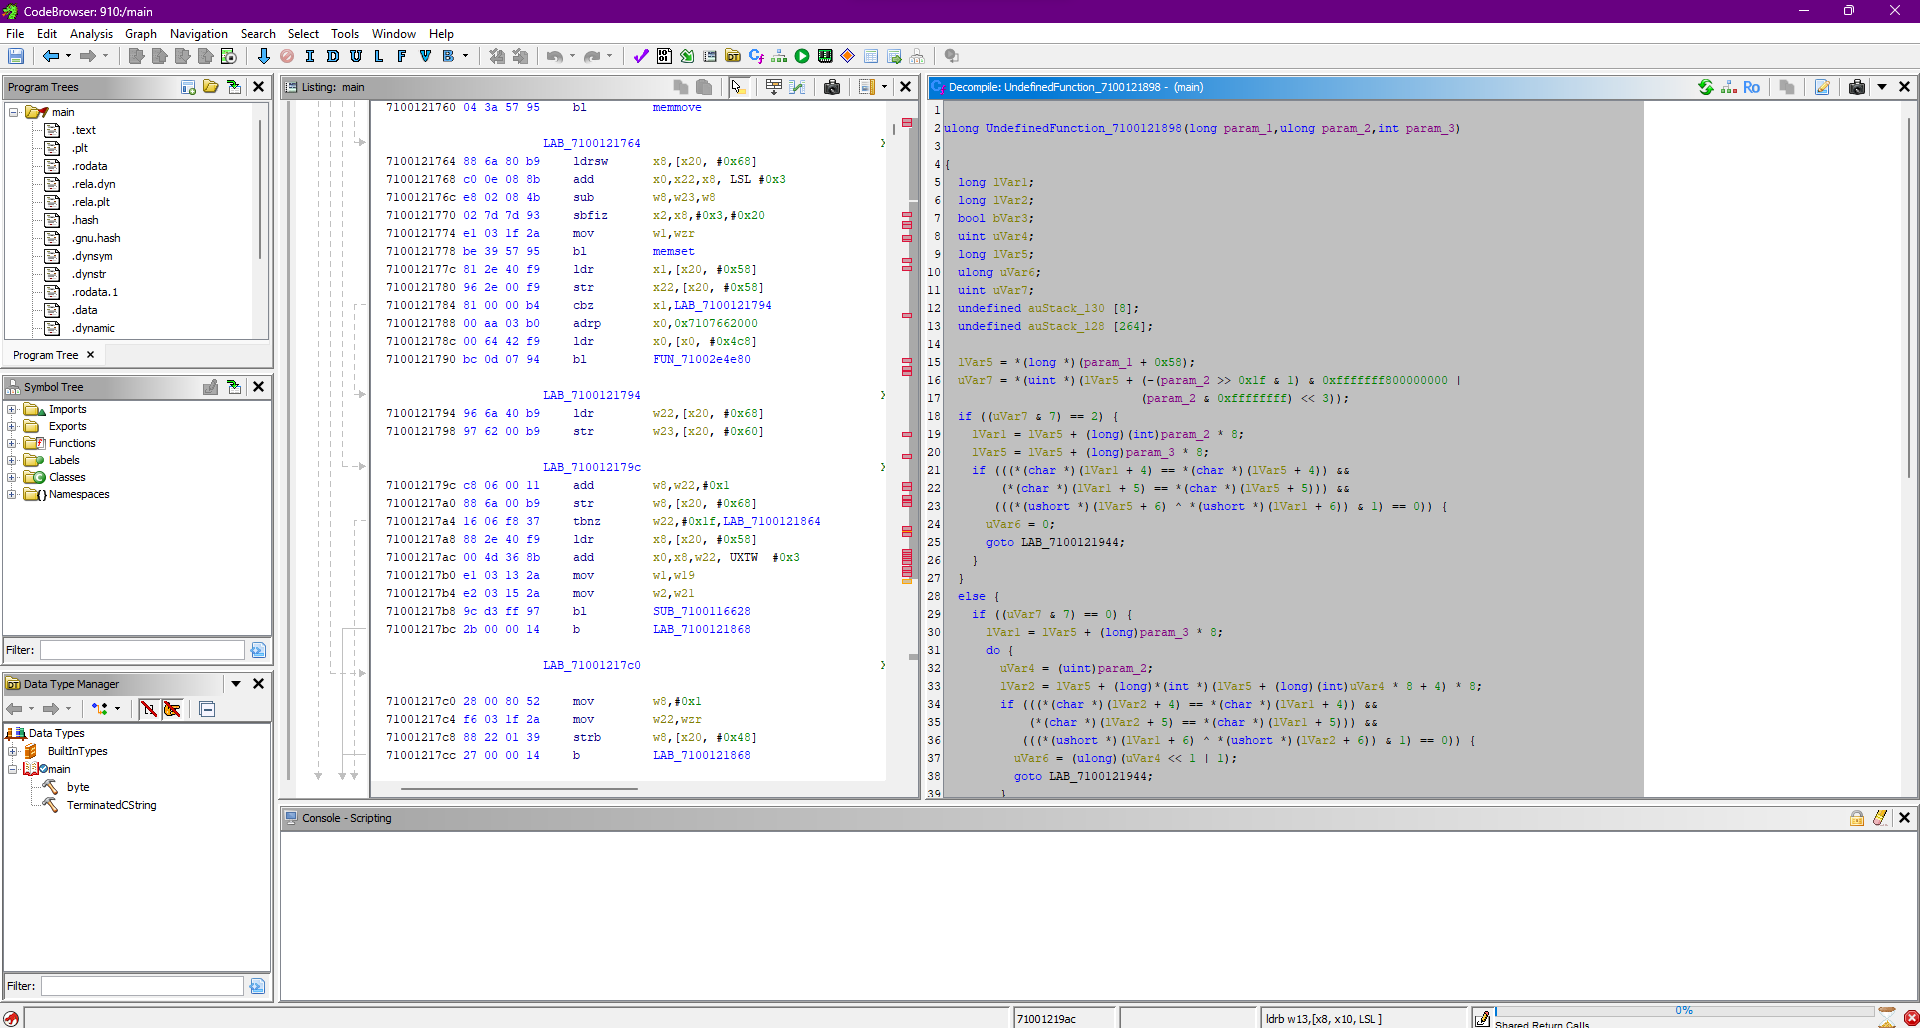
\includegraphics[width=\textwidth]{DecompiledAssembly}
        \caption {Decompiled Assembly Code}
        \label{fig:DecompiledAssemblyImage}
    \end{figure}

    \bigbreak
    \noindent
    The decompiled code below in \ref{fig:DecompiledAssemblyImage} does create C++ code, but without any parameter names, uses GOTO statements, and raw memory address accessing rather than any structs or class datastructures.
    The code did not create any functionality that does not exist in the assembly architecture used already.
    This exposed a gap in my knowledge where I didn't know how higher level concepts exist in assembly.
    Majority of the class had been spent discussing how concepts in higher levels translate into assembly in a more one-to-one fashion.
    In order to get a better understanding the decompiled code above, I would need to first learn how Object Oriented Programming principles exist in assembly, a language that notably does not do Object Oriented Programming.


    \section{Creating the Application}\label{sec:creating-the-application}

    \subsection{BlackJack.h \& BlackJack.cpp}\label{subsec:blackjack.h-&-blackjack.cpp}
    These two files contain a large amount of the logic regarding the overall game.
    The majority of complicated logic is done here, ensuring that any manipulation of strings and std::vectors is not handled in assembly code.
    While it is possible for \emph{some} of the logic here to be done in handwritten assembly, there were complications that prevented me from doing so.
    \bigbreak
    \noindent
    One of the issues I had found when working through this project is that the Microsoft Visual C++ Compiler and Linker do not allow for having multiple .cpp file equivalents per header file.
    This meant that I could not write a Class.h file to create a class definition, a Class.asm file to implement some of the member functions, and then also include a Class.cpp file to implement member functions that would prove too difficult to write in handwritten assembly.
    Because of this issue, I decided to focus my efforts on the Player class for assembly implementations, and leave the BlackJack class as a full C++ implementation.
    \bigbreak
    \noindent
    Doing so also allowed me to ensure that functions were actually be implemented fully correctly.
    If the BlackJack class calls functions of Player objects which are implemented in assembly, I can ensure that those class objects are being called correctly.
    If I were to implement \emph{all} functions only in assembly, then there is technically no guarantee that I am actually working with the classes on the assembly side the way that C++ expects to.
    Through leaving the BlackJack class only in C++, and calling Player functions normally as one would in C++, I guarantee that the functions I create in assembly truly are the implementations of the member functions C++ expects to be using.

    \subsection{Card.h \& Card.asm}\label{subsec:card.h-card.cpp-&-card.asm}
    Card.h contains several function and class definitions for needed utilities.
    Part of this is also the inclusion of the Suit enum.
    Originally, because the project was about seeing how different high level concepts compile down to assembly and being able to work with those, I had wanted to include an enum learn how those are implemented.
    However, during testing I had discovered that an enum converts directly to the datatype specified, similar to how const values or \#define statements operate.
    Because of this, I did not make it a priority to include enum functionality in the assembly code.
    \bigbreak
    \noindent
    Card.asm implements functions that operate on structures.
    The reason these functions exist is to ensure that functions implemented in one assembly file would still be use-able in other assembly files.
    Had I not been able to use the Card.h functions in Player.asm, regardless of their implementation location, the project would not be able to be completed.

    \bigbreak
    \noindent
    Also within Card.asm is another definition for the Card struct.
    During my testing, I was unable to find a struct used by the compiler to do calculations or checks using a Card object.
    This told me two things.
    Firstly, if I had wanted to be able to load the rcx register passed Cards into a struct, I would need to create that struct for myself.
    Secondly, the Microsoft Visual C++ Compiler, when compiling for structs, uses raw memory offsets rather than creating the structs.
    Both of these were valid options when writing handwritten assembly, however using the struct objects allows to ensure the offsets are correct and do not need to be changed should the actual datastructures change.
    Therefore, I elected to simply load card objects into structs.

    \bigbreak
    \noindent
    In order to be able to write the Card.h defined functions in assembly, they needed to first be imported into the assembly file.
    Rather than using the previous method, functionName PROTO, it would be done by using the PUBLIC keyword.
    So, to import the function ``int getCardValue(Card card)'' the correct line of code would be PUBLIC getCardValue.

    \bigbreak
    \noindent
    Card.asm
    \begin{figure}[hbtp]
        \begin{lstlisting}[language=MASM,label={lst:Cardasm}]
PUBLIC ?getCardValue@@YAHUCard@@@Z
PUBLIC  ?getCardValueString@@YADUCard@@@Z

sCard STRUCT
	value BYTE 0
	suit WORD ?
sCard ENDS

.data

card sCard < ?, ? >
        \end{lstlisting}
    \end{figure}

    \noindent
    However, in order to ensure I would be able to use classes properly, there is one thing that was omitted which caused extra problems, which would be name mangling.

    \subsection{Name Mangling}\label{subsec:name-mangling}
    As shown in~\ref{lst:Cardasm}, the names of the functions in the assembly code are not coherent.
    This is due to a concept known as ``Name Mangling.''
    It is best to explain this now, as it will become very apparent when discussing \ref{subsec:player.h-&-player.asm}.
    Name Mangling is the process in compiling code where functions and variables have their names programmatically changed to ensure there are no duplicate variable names.
    Variables and functions in assembly do not have scope, since after compiling into .obj files they are linked together, so it is important that all variables and functions have unique identifiers.

    \bigbreak
    \noindent
    This however, causes problems when trying to write implementations of these functions in assembly.
    While the mangled names \emph{are} programmatically created, they are not shown to the programmer without going through several hurdles first.
    In order to actually receieve the mangled names, there was a several step process.
    \begin{enumerate}
        \item Write the function definition in the Class Header file
        \item Create an empty function in the Class implementation file (.cpp file)
        \item Build the program
        \item In a terminal, navigate to the project output folder (in my case, it was ~/x64/Debug/)
        \item Run the command ``dumpbin /symbols Class.obj''
    \end{enumerate}
    This would dump all symbols found in the resulting file.
    However, assuming the class is one that uses external libraries such as $<$iostream$>$ or $<$string$>$, there would be too many symbols in the file to be able to find the ones that belong to your class implementation.
    In order to actually find the mangled names, it was easier to use the command ``dumpbin /symbols Class.obj $|$ Select-String `Class::' '' as it would filter the output of the dumpbin command to only the class's function definitions.

    \begin{figure}[hbtp]
        \centering
        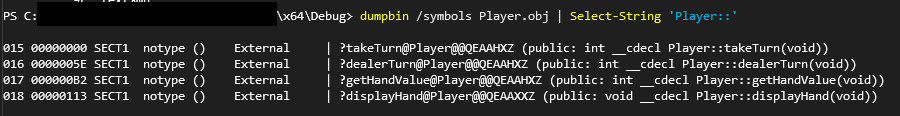
\includegraphics[scale=4]{dumpbin}
        \caption {Output of the dumpbin command on Player.obj}
        \label{fig:Dumpbin}
    \end{figure}

    \noindent
    Once these mangled names were found, they would be consistent so long as the function definition did not change.
    The mangled names often included some reference to the original function name and the class the function belongs to, if it belonged to one.
    Should the function definition change in any way, the entire process would need to be repeated to discover the new name of the function.

    \subsection{Player.h \& Player.asm}\label{subsec:player.h-&-player.asm}
    Player.h and Player.asm contain all code regarding a player's actions and the logic surrounding them.
    For the purposes of simplicity, the dealer is considered a player.
    Functions that handle input and output to the console are called from within the player's member functions.
    The player member functions also call other functions from the player class.

    \bigbreak
    \noindent
    In order to ensure this was possible, storing the `this' pointer into a reserved variable.
    It is possible to have done this by pushing and popping this value onto the stack, however saving it into an dedicated variable was more simple than dealing with stack operations.
    The reason this was required is because of how C++ handles member functions.
    Consider the following class definition example.

    \bigbreak
    \noindent
    Timer.h
    \begin{lstlisting}[language=C++,label={lst:TimerClass}]
class Timer {
public:
    Timer();

    // Display method
    void display();
    void update(float deltaTime);

private:
    float mTime;
}
    \end{lstlisting}

    \bigbreak
    \noindent
    the `display()' method takes no parameters when being called, and the `update(float deltaTime)' function takes one float parameter.
    However, secretly, this is not true.
    In C++, much like python if you have any experience with it, all member functions pass the `this' pointer in as the first parameter.
    Thus, the member function definitions could be thought of as looking like the following:
    \bigbreak
    \noindent
    Timer.h
    \begin{lstlisting}[language=C++,label={lst:TimerClassFunctionsWithThis}]
    void display(Timer* instance);
    void update(Timer* instance, float deltaTime);
    \end{lstlisting}

    \bigbreak
    \noindent
    When one of these functions is called, the memory address of the class instance the function is being called on is loaded into the instance parameter slot.
    In assembly, this is the rcx register.
    So, to ensure that the member functions are called properly, the memory address of the current class instance, what is known as the `this' keyword in C++, is preserved and loaded into rcx before each function call.



    \subsubsection{Extern ``C''}
    One question those with experience working with C$/$C++ and assembly might have is ``Why do you not simply use the Extern ``C'' keyword and avoid the class's Name Mangling all together?''
    To answer that, first recall what Name Mangling does from~\ref{subsec:name-mangling}.
    Name Mangling prevents the function name from being modified during the compilation of the C$/$C++ code.
    However, this does not work with class data structures.
    Consider the following class definition along with the one from~\ref{lst:TimerClass}.
    \bigbreak

    \noindent
    Thermometer.h
    \begin{lstlisting}[language=C++,label={lst:ThermometerClass}]
class Thermometer {
public:
    Thermometer();

    // Display method
    void display();

    void setTemperature(float temperature);
    float getTemperature();

private:
    float mTemperature;
}
    \end{lstlisting}

    \bigbreak
    \noindent
    Both class definitions contain a ``display()'' member function.
    This is allowed in C++ because of the functions' scopes.
    If the Extern ``C'' keyword were to be applied to each of those member functions, which would be the function called display?
    Functions cannot share names in assembly, so only one of them can be called `display' on the compiled assembly.
    Thus, disabling Name Mangling on member functions and member variables is not allowed to prevent this situation from occurring.

    \subsubsection{Variable Accessing}
    \noindent
    If you recall from, ~\ref{subsec:card.h-card.cpp-&-card.asm}, I had created a struct to place card objects into to access the structs variables consistently.
    There is no Player struct defined in Player.asm, so how are the actual card locations accessed?
    The player class was carefully constructed to ensure the offsets are correct and consistent.
    Similar to assembly structs, a class does not actually have a concrete memory address, contrary to what the ``this'' keyword in C++ would have you believe.
    Instead, structs and classes use memory offsets to find member variables, and the memory address of the class simply points to the first member variable in the class.

    \bigbreak
    \noindent
    When crafting the Player class, I ensured that the Card[] would be the variable that the memory address of the class points to.
    The only member variable in the Player class is a struct called a `Hand,' which acts as a container for a card array.
    This card array is also the first variable defined in the Hand struct, meaning that after all the struct abstraction, the memory address of the ``Player'' class truthfully points to a C++ char variable that holds the value of the first card.
    Then, accessing further cards in this array is the same as accessing any other value in an array, taking the memory address of the first element in it, and adding the index of access multiplied by the size of the object.

    \section{Download}\label{sec:download}
    The project in full can be downloaded from my \href{https://github.com/AKonicki26/CSI-370}{GitHub}.
    I recommend downloading the source code rather than any finished product as the motivation behind the project is on how the different source code elements link together rather than the actual finished product.

    \section{In Retrospect}
    With this project, I have accomplished what I set out to do.
    While there are improvements that could have been done, the focus of the project was on educational growth rather than the actual final deliverable.
    Discovering \emph{how} these functions will link together with the original class declarations had taken an unfathomable amount of time in a test class, before I had even started working on the Blackjack game itself.
    Had I had to do this project again, the only thing I would have done differently would be to choose a different implementation.
    Using the BlackJack method made it fairly overcomplicated.
    Because of the difficulty of using a game with random elements and a deck that needs to be shuffled before it can be accessed, there were many elements of the game I was unable to write in assembly.
    While it wasn't required to write \emph{all} code in assembly, I would have liked to do more of the game logic in assembly than just the Player logic.

    \bigbreak
    \noindent
    Regardless of the minuscule gripes I have, I am deeply proud of this project.
    If there is any major takeaway I will have from this class, it is how classes work at a fundamental level.
    Understanding the memory addresses of classes, the offsets they use, and how the functions don't actually exist as members of the class have elevated how I understand higher level programming languages dramatically.
    A large amount of the programming I do is in languages that use Object Oriented Programming principles.
    My language of choice is C#, a language that near \emph{requires} the use of Objects.
    Being able to have a better understanding of what is happening when classes are made, functions are called, and weird memory accesses happen will allow me to better work in the high level languages that use Classes often.

\end{document}